\section{Code generation}
%\subsection{Transformation pattern}
%todo: describe the pattern

%Transformation from State machine to fUML (classes, attributes, methods)
%\lipsum[1]

\subsection{Assumption}
%todo: give some assumptions on code generation such as functions to create methods, attriutes, classes
To give the formalization of the code generation, we assume that we want to generate from the state machine to an object oriented programming language $ActLang$. Assuming that our code generator contains primitive functions supporting for generating $ActLang$ as following:
\begin{itemize}
	\item $genClass(n, generals, itfs)$ creates a class with its name, parent class set, and implemented interfaces as \ti{n}, \ti{generals}, and \ti{itfs}.
	
	\item $genMtd(n, c, type, params)$ creates a method $m$ with its name as $n$ inside the class $c$, its return type as $type$, and $params$ as its parameter set.
	
	\item $genAttr(n, c, type, multiplicity)$ creates an attribute named $n$ in the class $c$ and typed by $type$. The create attribute is an array if $multiplicity > 1$, otherwise a simple attribute.
	
	\item $genEnum(n)$ and $genEnumLit(enum, n)$ create an enumeration and its enumeration literal, respectively.
	
	\item $genBody(m, body)$ adds a body to a method. The body is a string which contains a list of statements.
	
	\item $createParalle(t, seg)$ generates a mechanism which allows the segment code $seg$ run in a thread $t$. Similarly, $genWait(t), genJoin(t)$.
	
	\item $genMutex(size)$ creates an array of mutexes with \ti{size} as the number of items of the array. 
	
	\item $synchronize(seg)$ generates a mechanism which allows the segment code $seg$ run safely (can be either based on \ti{POSIX pthread} or \ti{Java synchronize} mechanism).
	
	\item $toString(stts)$ is used to convert a list of statements $stts$ into a readable string which can be add to a method as its body.
	
	\item Concatenation of two strings $str1$ and $str2$ is concisely described as $str1 + str2$.
	
	\item \ti{WHILE}, \ti{FOR} \ti{IF}, \ti{ELSE} are symbols representing while and for loops, if and else statements.
	
	\item \ti{FORK(func)} creates a thread (lightweight process) associated with the function/method \ti{func} and \ti{JOIN(theThread)} waits until the method associated with the thread \ti{theThread} completes.
\end{itemize} 

\subsection{Code generation algorithm}
\subsubsection{State transformation}
Suppose that we want to generate a state machine $sm$ whose states are listed by $lstates$. A common state interface $IState$ is created. The interface contains three methods, namely, \ti{entry}, \ti{exit}, and \ti{doActivity} corresponding to three state actions, respectively. To preserve the hierarchy of composite states, the interface also has two attributes called \ti{activeStates} and \ti{previousStates} referring to active sub-states \ti{actives} , previous active sub-states \ti{previousStates} in case of the presence of history states, and a list of deferred event identifiers.

Each UML state is transformed into an instance of the interface associated with a state ID (which is a child element of an enumeration) inside the active class $C$. When initialization, each instance refers its methods to the actual methods implemented in $C$. In C++, this referring is done by using the powerful mechanism function pointer. In other object-oriented languages such as Java, this is done with anonymous sub-classes of the interface. Listing \ref{lst:IStateCpp} and \ref{lst:IStateJava} show the interface and its instances associated with the states of the state machine in C++ and Java, respectively, in which S0 is one of $lstates$. \ti{NUM\_STATES} is the number of states in the state machine. The actions of the states are implemented in the active class $C$ and named depending on the name of the states. In the following sections, we only consider C++ as out \ti{ActLang}. The discussion of other object-oriented languages are much similar since these share the same concepts,  

\begin{lstlisting}[caption=IState interface and function pointers in C++, label=lst:IStateCpp, frame=single]
typedef struct IState {
  IState** previousStates; 
  IState** actives;
  EventId* defEvents;
  void (C::*entry)();
  void (C::*exit)();
  void (C::*doActivity)();
} IState;
class C {
private:
  IState states[NUM_STATES];
public:
  C() {
    states[S0_ID].entry = &C::S0_entry;
    ...
  }
  void S0_entry {...}
}
\end{lstlisting}

\begin{lstlisting}[mathescape=true, caption=IState interface and annonymous sub-classes in Java, label=lst:IStateJava, frame=single]
public interface IState {
  public IState[] previousStates; 
  public IState[] actives;
  public EventId defEvents;
  public void entry();
  public void exit();
  public void doActivity();
}
class C {
private IState states[NUM_STATES];
public C() {
  states[S0_ID] = new IState() {
    public void entry() {
      S0_entry();
    }
    ...
  }
}
public void S0_entry() {...}
}
\end{lstlisting}

The procedure to generate the code for states is shown in Listing \ref{lst:procedure1}. It first creates the state interface $IState$ (in C++, it is either a class or a struct). The array attribute is then created with the number of states as its size. Each state is also associated with a state ID which is a child of an enumeration. Finally, the constructor of $C$ is created to initialize and make methods of the attribute instances refer to \ti{entry/exit/doActivity} action methods of $C$. The implementation of action methods in the context class $C$ is similar to the delegation pattern proposed by the authors in \cite{Niaz2004} but dramatically decreases the memory consumption since only one common interface for all states is created instead of a class for each state in \cite{Niaz2004}.

\begin{lstlisting}[mathescape=true, caption=Procedure to create code for states, label=lst:procedure1, frame=single]
IState = genClass('IState', $\emptyset$, $\emptyset$);
stateIdEnum = genEnum('StateIdEnum');
foreach s in lstates
  genEnumLit(stateIdEnum, s.name + '_ID');
  mtd = genMtd(s.name + '_entry', C, 
			null, null);
  genBody(mtd, toString(entry(s)));
  ...
genEnumLit(stateIdEnum, 'NUM_STATES');  
genAttr('states', C, IState, NUM_STATES); 
genMtd(C.name, C, null, null);
\end{lstlisting}

\subsubsection{Region transformation}


\subsubsection{Event transformation}
An event enumeration \ti{EventId} is created whose children are event identifiers associated with events. Each event is also transformed into a method in the context class $C$. Suppose $levents$ is the list of events which can be processed by the state machine $sm$. Besides the explicitly defined events of the state machines, $levents$ contains a special event called $CompletionEvent$. The latter is, following the UML specification, an implicit event triggering triggerless transitions. It is emitted when either \ti{doActivity} of an atomic state finishes its execution or all orthogonal regions of a composite state have reached to a final state. 

UML defines five types of events including \ti{CallEvent}, \ti{SignalEvent}, \ti{TimeEvent}, \ti{ChangeEvent}, and \ti{Any}. A transition triggered by an \ti{Any} event is meant to be fired by any of the other events. To process events, for each event, a method is implemented in $C$. Each event triggers a list of transitions. We suppose $T_{trig}(e)$ is the transition list triggered by the event $e$, and $S_{trig}(e) = \{src(t) | t \in T_{trig}(e)\}$. In other words, $S_{trig(e)}$ is a set of states which are the source states of the transitions in $T_{trig}(e)$. To present how the body of event methods is generated, we define functions as followings:
\begin{itemize}
	\item Vertex depth $dp(v)$ is defined as:
			\begin{equation}
			dp(v) =    \left\{
			\begin{array}{ll}
			1 & \ti{v is a root vertex}  \\
			dp(ctner(v)) + 1& otherwise \\
			\end{array} 
			\right.
			\end{equation}
	\item $Map_{e}(s) \subset S_{trig(e)} | \forall sub \in map_e(s): ctner(sub) = s$, $Prt(e) = \{s \in V| map_{e}(v) \neq \emptyset\}$. $Prt(e)$ is an ordered list whose length is $len(Prt\{e\})$ and elements are accessed by indexes. The order of $Prt(e)$ is defined as:	$\forall i, j \leq len(Prt\{e\})$, 
	\\ if $i < j, dp(Prt(e).get(i)) \geq dp(Prt(e).get(j))$. 	
\end{itemize}


The procedure in Listing \ref{lst:eventproc} describes how to generate the body of the method associated with an event. It generates the code checking for active states respecting the UML semantics in which the innermost states process the incoming event first. To do this, it first looks in the source state list $S_{trig(e)}$ for the innermost states that accept the event triggering its outgoing transitions. If these found states are children of a concurrent state, $genStateCheck$ generates the checking codes run in parallel, which will be described later in \ref{subsubsec:thread}. Otherwise said, sequential code is generated.

\begin{lstlisting}[mathescape=true, caption=Procedure to create code event processing, label=lst:eventproc, frame=single]
for item in $Lm(e)$
  if ($item.kind = conc$)
    for s in Map_e(item)
      genStateCheck() 
  else 
    for s in Map_e(item)
      genStateCheckWithElse  	
\end{lstlisting}



\subsubsection{Thread-based Concurrency}
\label{subsubsec:thread}
\paragraph{Thread-based concurrency analysis} 

While concurrency is an important aspect defined by the UML State machine specification, especially hierarchical and concurrent state machines with \ti{doActivity}s for states, most of existing approaches do not take into account. This is non-trivial since concurrency is dynamic in UML state machine since the number of threads used for concurrency is non-deterministic.

For example, assuming that \ti{Idle} is the current active state of the ATM state machine in Fig. 
\ref{fig:example} and a \ti{verifyPIN} event is coming. 
The \ti{doActivity} behavior of \ti{Idle} \ti{doActivity(Idle)} (if has) is terminated, \ti{exit(Idle)} and the \ti{effect(t2)} (\ti{T2Effect}) are executed sequentially. 
These actions are run in a state machine main thread which reads incoming events from a "first in, first out" (FIFO) priority queue. 
Fig. \ref{fig:threading1} shows the activity diagram representing the concurrency of the state machine example when processing the \ti{verifyPIN} event, in which each activity partition represents a thread. 
The completion of \ti{effect(t2)} is followed by \ti{effect(t3)} and \ti{effect(t3)}, which are run concurrently since the transitions owning these effects outgo from a fork pseudo state. 
Two threads \ti{T3Run} and \ti{T4Run} associated with \ti{effect(t2)} and \ti{effect(t3)}, respectively, are created by \ti{FORK}.
The entry action \ti{entry(Verifying)} of \ti{Verifying} is executed following the termination of the two threads. 

After \ti{entry(Verifying)} completion, the UML specification says that \ti{doActivity(Verifying)}, \ti{entry(VerifyingCard)} and \ti{entry(VerifyingPIN)} should be concurrently executed, which is represented by a fork node, in which a \ti{Start} signal is sent to \ti{VerifyingDoRun} in order for commencing \ti{doActivity(Verifying)}. 
As the \ti{Verifying} state, the \ti{doActivity}s of the states \ti{VerifyingCard} and \ti{VerifyingPIN} are also concurrently started. 
Also, upon the completion of \ti{entry(VerifyingCard)} and \ti{entry(VerifyingPIN)}, the main thread completes the processing of the \ti{verifyPIN} event, reads next events from the queue or waits for next event occurrences.

\begin{figure}
	\centering
	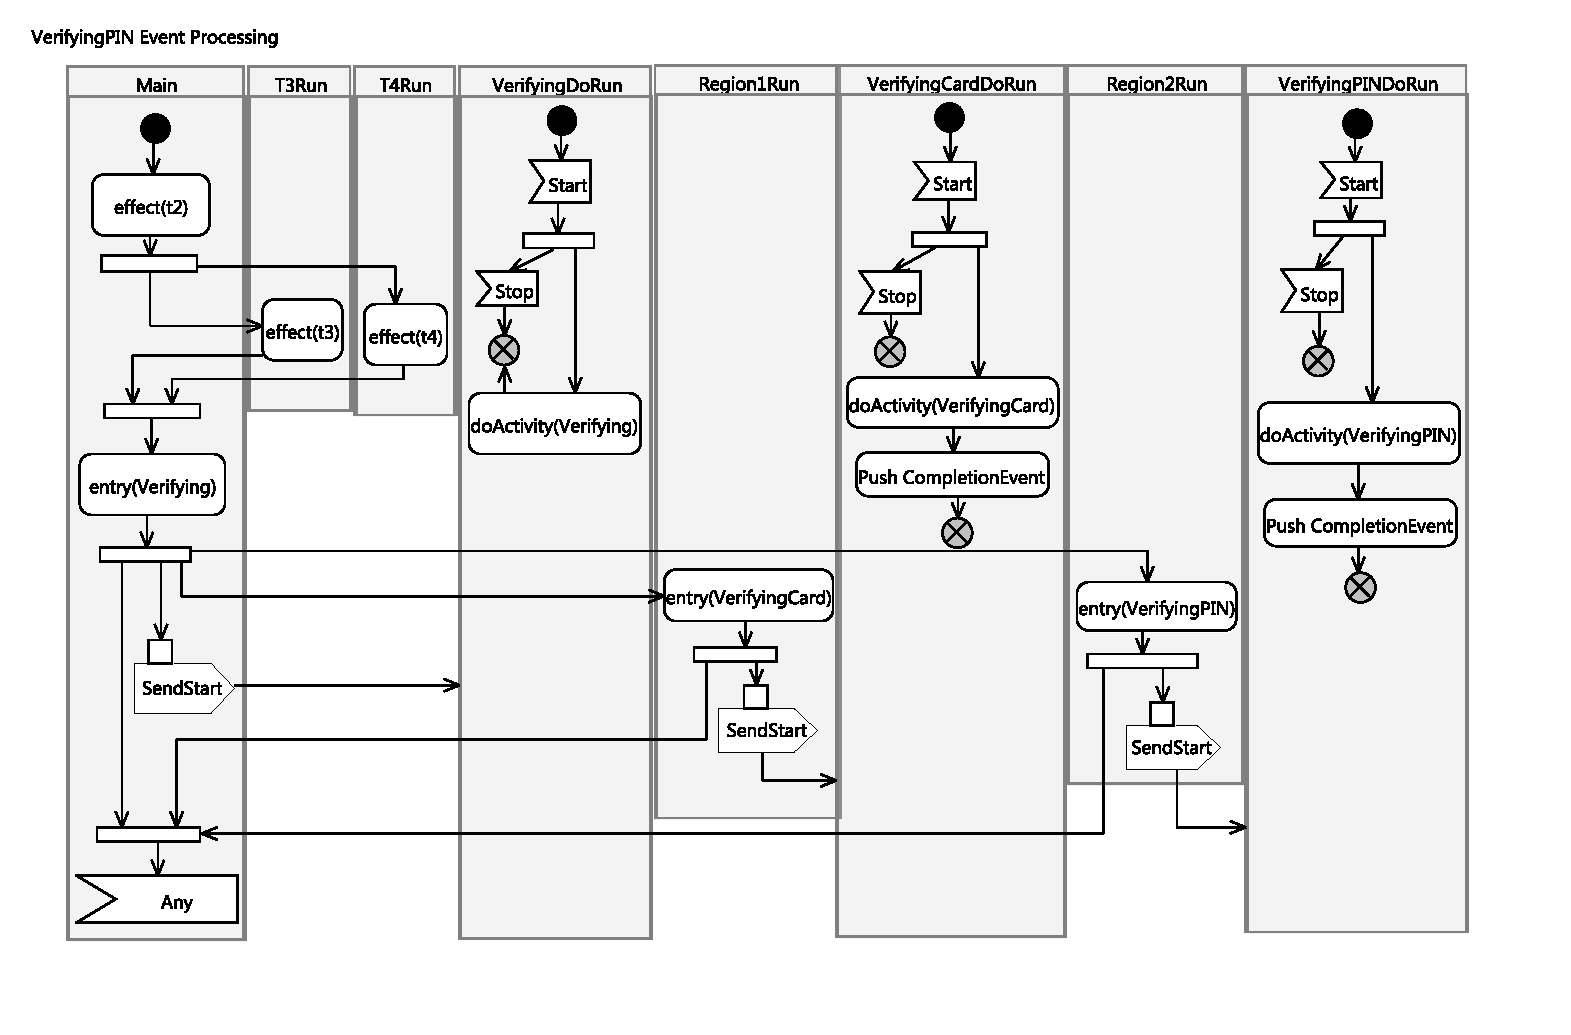
\includegraphics[clip, trim=1.0cm 1.6cm 1.6cm 1cm, width=1.03\columnwidth]{figures/ThreadingExample.pdf}
	\caption{Concurrency of the ATM when receiving the \ti{verifyingPIN} event} 
	\label{fig:threading1}
\end{figure}

If no event is coming, and \ti{doActivity(VerifyingCard)} and \ti{doActivity(VerifyingPIN)} are long actions (e.g. forever loops inside), the state machine remains its active configuration and three concurrent actions including \ti{CheckForEvents}, \ti{doActivity(VerifyingCard)}, and \ti{doActivity(VerifyingPIN)} are permanently run.

It is worth noting that the termination time of \ti{doActivity(VerifyingCard)} and \ti{doActivity(VerifyingPIN)} is non-deterministic. 
However, whenever one of those completes, a completion event associated with the state corresponding to the completed \ti{doActivity} is generated and pushed to the event queue. 
For illustration, assuming that \ti{doActivity(VerifyingCard)} terminates before \ti{doActivity(VerifyingPIN)}. 
As the activity diagram in Fig. \ref{fig:threading2}, the Main thread checks the \ti{CompletionEvent} upon the completion of \ti{doActivity(VerifyingCard)}. \ti{exit(VerifyingCard)} and \ti{effect(t5)} are then executed sequentially. If \ti{cardValid} is computed as true as the result of \ti{doActivity(VerifyingCard)} and \ti{exit(VerifyingCard)}, the Main thread simply executes \ti{effect(t6)} and \ti{entry(CardValid)} before waiting for other events.

In contrast, Main sends \ti{Stop} signals to stop \ti{doActivity(VerifyingPIN)} and \ti{doActivity(Verifying)}, executes exit actions, effects and entry actions in an appropriate order (see Fig. \ref{fig:threading2}) and waits for other events.

So far, we see that the number of concurrent actions is not constant but changes timely. 
Each action can either deterministically or non-deterministically terminate. 
In this sense, deterministic actions (DAs) prevent the Main thread from going to the waiting-for-event point. 
In other words, pending events in the queue are only read and processed once all deterministic actions complete. Therefore, we re-define the run-to-completion paradigm of UML state machine as following:
 
\begin{definition}
	Run-to-completion means that, in the absence of exceptions or asynchronous destruction of the context	class object or the state machine execution, a pending Event occurrence is dispatched only after the completion of all deterministic actions commenced by the processing of the current event. 
	At this point, a stable state configuration has been reached
\end{definition}

In the example, some of DAs are as followings: \ti{effect(t2)}, \ti{effect(t3)}, \ti{effect(t4)}, \ti{entry(Verifying)}, \ti{entry(VerifyingCard)}, \ti{entry(VerifyingPIN)} and non-deterministic actions (NDAs) as followings: \ti{doActivity(Verifying)}, \ti{doActivity(VerifyingCard)} and \ti{doActivity(VerifyingPIN)}.


\begin{figure}
	\centering
	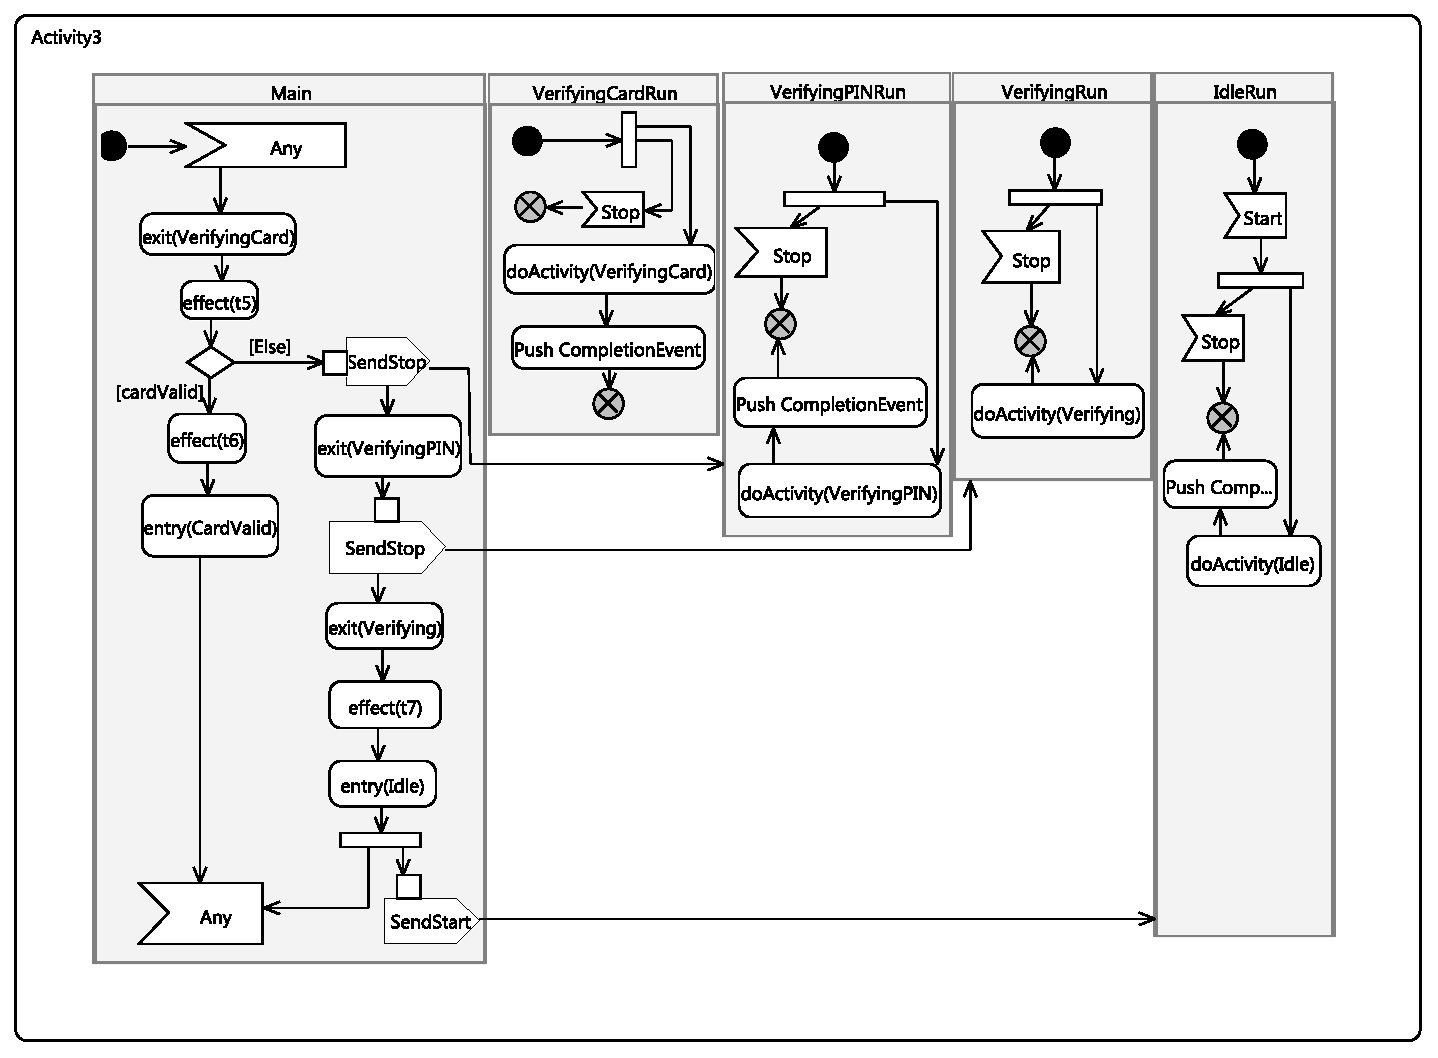
\includegraphics[clip, trim=1.5cm 1.6cm 1.6cm 1cm, width=1.03\columnwidth]{figures/ThreadingExample2.pdf}
	\caption{Concurrency of the ATM when \ti{doActivity} of \ti{VerifyingCard} completes before that of \ti{VerifyingPIN}}
	\label{fig:threading2}
\end{figure}

\paragraph{Thread-based design of generated code}
Each NDA is run in parallel with the main thread which reads and dispatch events from the event queue. 
Each is associated with a thread which is initialized at the state machine initialization moment. 
The number of threads associated with NDAs is therefore equal to that of the NDAs.
The design of threads is based on the thread pool pattern, which initializes all threads at once, and the paradigm "wait-execute-wait". 
In the latter, a thread \tb{waits} for a signal to \tb{execute} its associated method and goes back to the \tb{wait} point if it receives a stop signal or its associated method completes. 
An NDA is one of the followings:
\begin{itemize}
	\item \ti{doActivity} of each state if has. The number of \ti{doActivity} $n_{do} = \#\{s \in V|\exists doActivity(s)\}$
	
	\item Sleep function associated with a \ti{TimeEvent} which counts ticks and emits a \ti{TimeEvent} once completes: $n_{te} = \#\{e \in E|\ti{e is a time event}\}$.
	
	\item Change detect function associated with a \ti{ChangeEvent} which observes a variable or a boolean expression and pushes an event to the queue if changes happen: $n_{che} = \#\{e \in E|\ti{e is a change event}\}$.
\end{itemize} 

Therefore, the concurrency has the number of initial threads $n_{threads} = n_{do} + n_{te} + n_{che}$ plus a main thread which sends start and stop signals to these initial threads. 

Now we consider spontaneous threads which are created by \ti{FORK} to run DAs, joined until and destroyed once DAs complete. The followings describe different types of DAs:

\begin{itemize}
	\item Actions executed when entering/exiting an orthogonal region, which can be: execute a chain of transition effects contained by the region before entering a stable sub-state or exiting the region completely: $n_{region threads} = \#\{r \in \mathcal{R}|ctner(r).kind=concurrent\}$
	
	\item Effects of transitions outgoing from a $fork$ and those incomings to a $join$: \\
	$\mathcal{J} = \{v \in V|v.kind=join\}$ \\
	$\mathcal{F} = \{v \in V|v.kind=fork\}$ \\
	$$n_{FJ\_threads} = \sum_{v \in \mathcal{F}} {\#T_{outs}(v)} + \sum_{v \in \mathcal{J}} {\#T_{ins}(v)}$$.
\end{itemize}

The spontaneous threads follow a paradigm in which if a thread $parent$ creates a set of threads $children$, $parent$ must wait until $children$ complete their associate methods. These threads are created in one of the following cases:

\begin{itemize}
	\item Having multiple transitions outgoing from a \ti{fork}, for each transition effect, a thread is created by \ti{FORK}
	
	\item Entering a concurrent state $s$, after the execution of $entry(s)$, a thread is also created for each orthogonal region. 
	
	\item Exiting a concurrent state $s$, before the execution of $exit(s)$, a thread is also created for each region to exit the corresponding active sub-state. 
\end{itemize}

\paragraph{Example of generated code}

 


 

